
\section{Introduction}
Faceted browsing is ubiquitous on the Web today. Most if not all major online shops and media (video, images and music) platforms provide at least some degree of faceted browsing features to
navigate their products - or more specifically: the data records about them. Typical examples include support for filtering videos by length, music by genre, or generally products by relevant features[
%as shown in \autoref{fig:faceted-browsing-demo}. 
Conceptually, in many cases the underlying data can be seen as knowledge graphs (KG), i.e. entities and values are represented as nodes, and labelled edges are used to specify their semantic relation. In cases where data is modelled using RDF (and ontologies), it already forms a knowledge graph. In this case, SPARQL\footnote{\url{https://www.w3.org/TR/sparql11-query/}} is a standard language for uniformly querying instance and schema information.

In this paper, we present our SPARQL-based faceted browsing benchmark generation framework, designed to generate realistic faceted browsing scenarios on arbitrary data sets and assess triple store performance in regard to the faceted browsing paradigm.
%\todo{set-theoretic approach}
%Motivation
%- several faceted browsing systems
%  focus on user interfaces
%  - or generic benchmark with focus on triple store performance
%  - but with these approaches, to what extend user exploration via sparql works remains a mystery.
%- most if not all benchmarks require specific data sets - hard to evaluate one's own use case

Our contributions are as follows:
\begin{itemize}
    \item A highly flexible, schema-agnostic SPARQL-based faceted browsing benchmark generation framework
    \item Configurable benchmark generation based on chokepoints and user-provided data sets
%    \item Investigation of current limitations of real-time SPARQL-based faceted browsing
%    \item Evaluation of the schema-based path finding component used in benchmark generation
    \item Performance and correctness evaluation of contemporary triple stores using the HOBBIT benchmarking platform
\end{itemize}

Our resource is available at \\ \url{https://github.com/hobbit-project/faceted-browsing-benchmark}.

The remainder of the paper is structured as follows:
In~\autoref{sec:preliminaries}, we introduce the RDF and SPARQL and on this basis define the important notions.
Afterwards, in ~\autoref{sec:architecture}, we present the overall architecture of our system. The main building blocks are the faceted search query generation system and a component for schema-based path finding along properties, which are described in~\autoref{sec:engine}.
The benchmark generator itself is presented in~\autoref{sec:benchmark-generator}.
Our findings are reported on in~\autoref{sec:evaluation}.
We discuss related work in~\autoref{sec:related-work}. Finally, we conclude in~\autoref{sec:conclusions} and where we also point out directions for future work.

%\subsection{Resources}
%- Links to all resources:
%- Benchmark Generator
%- Generated Benchmarks
%- Hobbit Platform

%\section{Preliminaries}
%RDF, SPARQL, BGP

%In~\autoref{sec:engine} we present our SPARQL-based faceted search %engine, which is a fundamental building block of benchmark %generation system.

\section{Preliminaries}
\label{sec:preliminaries}
%The engine is data-driven, which means that facets and facet values correspond directly to the available properties and property values, respectively, in an RDF dataset.

\subsection{RDF and SPARQL}
The Resource Description Framework (RDF) is a W3C standard for data interchange\footnote{\url{https://www.w3.org/RDF/}}.
The most fundamental introduced entity is the \emph{RDF graph} which conceptually is a set of triples.
A triple can be seen as a labelled ``link'' between two nodes.

Formally, let there be sets of IRIs $I$, blank nodes $B$ and literals $L$. Further, let the set of
\emph{RDF term}s $T := I \cup B \cup L$.
An \emph{RDF Graph} $G$ is defined as $G \subset (I \cup B) \times I \times T$.

Although RDF graphs are often depicted as conventional labelled graphs, they are formally defined of ternary relations which in turn correspond to directed labelled pseudo graphs. Pseudo graphs allow for multiple edges
to exist between a given pair of nodes, as well as for the same node to act as the start and end of an edge.
Hence, in some cases commonly used graph algorithms may not be applicable to given RDF data.
% Vocabularies

SPARQL (a recursive acronym for \emph{SPARQL Protocol and RDF Query Language})
is a W3C standard that devises protocols and languages for querying and updating RDF.
Our benchmark generator will produce SPARQL queries that correspond to faceted search and browsing operations on an RDF data set. The generated benchmarks can be executed on any system implementing SPARQL.
% Graph pattern
%Triple stores


\subsection{Paths}
With SPARQL 1.1, \emph{property paths} expressions were introduced to the query language.
Since then it is possible to query a data set for all pairs of resources connected via sequences of RDF predicates that match a given path expression. For instance, \emph{?sub rdfs:subClassOf* ?super}
will yield any pair of resources reachable by zero-or-more forward traversals along the \emph{rdfs:subClassOf} predicate.
For our work, we introduce the notion of \emph{simple (property) paths} as (possible empty) sequences of \emph{steps} which are (predicate, direction) pairs. Direction is either \emph{forwards} or \emph{backwards}.


%Further, we introduce the following notions, which in the case of empty paths all yield \emph{nil}.
%\begin{itemize}
%  \item $parent(path)$ yields the parent path (i.e. the path with the last step omitted).
%  \item $reachingPredicate: P \rightarrow I$ yields the (predicate) IRI by which the path's destination is reached, i.e. the last predicate of a path.
%  \item $reachingDirection: P \rightarrow D$ analogously yields the direction of the last step.
%\end{itemize}

%We introduce the notion of an \emph{arrow} as a pair combining a path with direction.\footnote{One can think of the path
%acting as the shaft, and the direction as the tip.}

\subsection{Node-centric Sparql Queries}
\begin{lstlisting}[language=sparql, label=lst:pquery, caption=Pseudo code for a node-centric query and property access]
NodeCentricQuery
  .from(
      CONSTRUCT WHERE {
          ?employee :employedAt ?department ;
                rdfs:label ?l 
      })
  .partitionBy(?employee)
  .executeOn(sparqlEndpoint)
  .forEach(rdfNode -> rdfNode.getProperty(rdfs:label))
\end{lstlisting}
\emph{CONSTRUCT} is a standard SPARQL query form which allows for retrieval of RDF graphs. However, many use cases do not demand for a single monolithic RDF graph,
but rather individual partitions that form logical objects that can be processed independently.
For example, a query about employees and departments may look like \autoref{lst:pquery}.
From the query alone, one cannot deduce whether it is department-, employee- or triple-centric.
However, if we denoted e.g. \emph{?department} as a \emph{partition} variable, we can easily group triples
based on this condition for further processing.
A \emph{node-centric SPARQL query} is thus simply a pair comprised of a standard construct query and a single partition variable.
Partitioning could also be applied to \emph{SELECT} queries, however, in the case of \emph{CONSTRUCT}, access of retrieved data becomes object-like. %, and thus exhibits benefits:
%Similar to as one would access properties of e.g. a JSON object, one can -- starting from a binding of one of the partition variables %--
%access its retrieved predicates, as sketched in~\autoref{lst:pquery}.
Note, that the construct template may be empty, in which case the result is a set of RDF terms (such as literals) with no related triples.
% aspect is, whether to treat each instance of the CONSTRUCT template as an object, or 
%In fact, the Apache Jena framework\footnote{\url{https://jena.apache.org/}} features tooling to 

In our work, we use this mechanism for obtaining facet values and counts.

\section{Framework Architecture}
\label{sec:architecture}

\begin{figure}
\centering
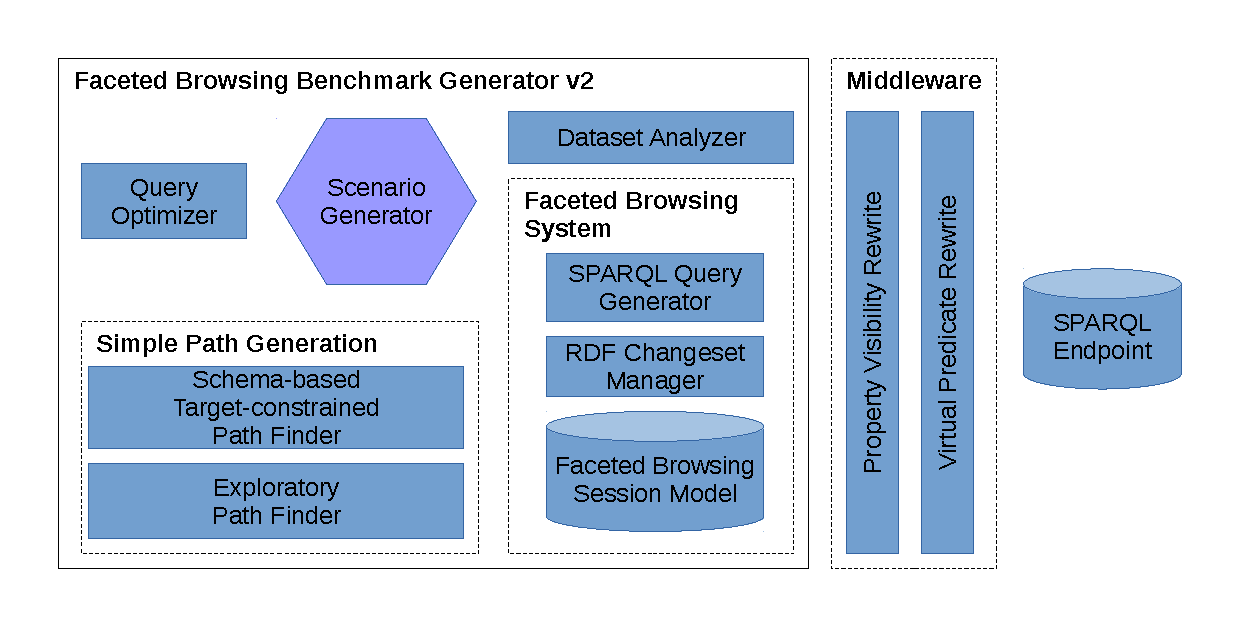
\includegraphics[width=\textwidth]{images/Architecture}
\caption{Architecture of the Schema-agnostic SPARQL-based Faceted Browsing Benchmark Generation\label{fig:architecture}}
\end{figure}

\autoref{fig:architecture} depicts the components of our faceted browsing benchmark generation system, which we briefly explain below: 
\begin{itemize}
\item The \emph{Scenario Generator} drives the benchmark generation and uses the APIs and services provided by the other components.
A scenario is a sequence of faceted browsing interactions.
\item The \emph{Dataset Analyzer}'s purpose is to obtain metadata about a data set. Most relevant to us are the used predicates and their ranges, and the schema-graph, i.e. which instance types are connected by which properties.
%(see \autoref{sec:dataset-analysis}).
This metadata is used by the path finder sub-system.
\item The \emph{Exploratory Path Finder} tries to generate -- starting from a set of resources -- simple paths that meet given specifications.
\item The \emph{Schema-based Target-constrained Path Finder} is used to find simple paths that end in a given set of predicates, such as a numeric one or a pair that represents longitude and latitude. This component uses the schema-graph to generate candidate paths. %The system under test (SUT) SPARQL endpoint is then queried for whether there are actually resources connected by the candidate paths.
\item The \emph{Query Optimizer} is used to post-process generated SPARQL queries in order to make them more natural as if they were written by a human expert.
For instance, whenever possible, variables in triple patterns are substituted with constants and filter expressions are simplified. This has two purposes: On the one hand it relieves the work of query optimiser when testing the benchmark on target SPARQL systems.\footnote{Example issue that was mitigated by improving our own query optimiser: \\ \url{https://github.com/openlink/virtuoso-opensource/issues/822}}
\item The \emph{Middleware Layer} is the place where certain virtual data transformations relevant to faceted browsing can be implemented using query rewriting. (It is not part of the Benchmark Generator.) % Some triple stores support these rewriting features natively, whereas our framework provides limited triple-store-independent implementations.
%, whereas our framework also ships with prototype implementations. %integrated.
%we created prototype implementations which are summarized here for completeness:
%  \begin{itemize}
%  \item \emph{Property Visibility}: In many cases, it is undesired to have all predicates of a dataset to show up as facets in a faceted browser.
%  This component can hide predicates by means of injecting appropriate FILTER statements into SPARQL queries based on given whitelists or blacklists.
%  \item \emph{Virtual Predicate Rewrite}: Sometimes predicates desired to appear in a faceted browser are not directly present in a dataset.
  For example, browsing people by \emph{age} may feel more natural than by \emph{birth date}. In a data set, typically the latter predicate is preferred as it refers to static information, whereas the former one changes every year. This rewrite component allows one to define custom virtual predicates using SPARQL queries.    
%  \end{itemize}
\end{itemize}


\section{SPARQL-based Faceted Browsing System}
\label{sec:engine}
The most fundamental component of our benchmark system is unsurprisingly the faceted browsing system.
It provides the means necessary to interact with an RDF dataset according to the faceted browsing paradigm.
First, we present a domain-specific language for expressing faceted queries. Subsequently, we show how they are translated to SPARQL.
%The faceted browsing engine is one of the two core building blocks of HFBBG. 

\subsection{A domain-specific language for Faceted Search}
In this section, we present a domain-specific language (DSL) for the implementation of a faceted search system.
The main idea is as follows:

Given an intensional description of a set of resources, e.g. all subjects of an RDF graph or all instances of type person. We now need mechanisms to obtain information about them, navigate along their properties to related set of resources, and apply constraints on these sets. In principle, this corresponds to building a SPARQL basic graph pattern by starting with a \emph{root variable}, and adding appropriate connecting \emph{triple patterns} and \emph{filters} as query generation progresses.

The entry point to the system is the \emph{FacetedQuery}. It is modelled with the following parts:
\begin{itemize}
\item A \emph{base SPARQL concept} that denotes the initial set of resources. Typically it denotes all of an RDF graph's subjects, but
it could also be set to e.g. the instances of a certain class or the set of predicates.
\item A set of (facet) \emph{constraints} - We represent constraints as SPARQL expressions, however, with a level of indirection: Instead of using (final) variables directly, references to \emph{FacetNode} or \emph{FacetMultiNodes} (explained below) are used. In the query generation phase, these references are substituted with the corresponding variables.

%entities that represent traversals of the data.
%Essentially, these traversals are simple paths.
%These traversals entities are internally created when trav
%FacetNodes and FacetMultiNodes.
%The type of the traversal determines whether multiple constraints are to be combined using conjunctions or disjunctions.
\item The \emph{focus}
%is a designated \emph{FacetNode} that
denotes the set of resources that serve as the base for facet value counts computations, in other words the base of the resources on display.
%Note, that despite constraints being SPARQL expressions, they are not injected into final SPARQL query directly:
%One the one hand, every reference needs to be resolved to its final variable and graph pattern,
%On the other one, additional transformations may be required, such as converting a spatial constraint involving a bounding box into the appropriate vocabulary and/or SPARQL dialect, such as WGS84, GeoSPARQL or Virtuoso's flavor of it.
\end{itemize}

\begin{figure}
\centering
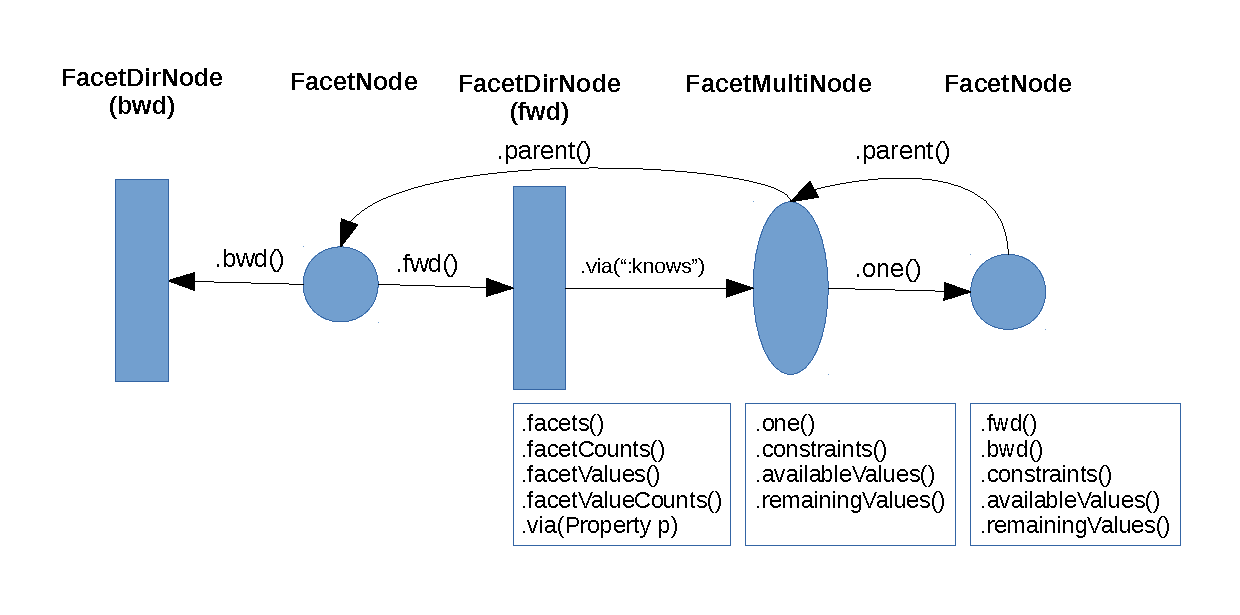
\includegraphics[width=\textwidth]{images/NodeModel}
\caption{The most relevant entity types and methods of the Faceted Browsing System. They enable traversal of a the data as well as retrieval of faceted-search-related information, such as available values or facet value counts.}
\label{fig:faceted-browsing-api}
\end{figure}
The focus of a FacetedQuery is a designated \emph{FacetNode}, whose related interfaces are depicted in~\autoref{fig:faceted-browsing-api} and are described as follows:
\begin{itemize}
\item A \emph{FacetNode} instance can be seen as a specific variable in a BGP  and thus intensionally represents a set of resources.
Using the \emph{.fwd()} or \emph{.bwd()} methods, one obtains a \emph{FacetDirNode} entity that represents the set of facets and facet values
reachable either in forward or backward \emph{direction}. 
%Note, that in principle a FacetNode could provide the functionality to access the union of both traversals, however we leave that for future work.
%Note, that presently a FacetNode does not directly support retrieval of facets and facet values.
%Instead, one first has to 
 
\item \emph{FacetDirNode} An intermediate entity for access to all facets in either forward or backward direction, backed by the \emph{immediate} triples of the resources represented by the FacetNode.
The methods \emph{availableValues} yields \emph{all} values from which constraints can be created, whereas \emph{remainingValues} yields
all values that do not yet satisfy any existing constraint. The latter method is used in our benchmark in order to create non-subsumed constraints. 
The FacetDirNode interface allows for forward and backward traversals via RDF predicates.

\item \emph{FacetMultiNode} An entity representing all SPARQL variables reached via the same origin and predicate.
Conjunctive constraints are managed here, and each addition of a constraint results in a new FacetNode -- and thus underlying SPARQL variable -- to
be allocated.
%\todo{probably re-add keyword example}
The \emph{primary} FacetNode -- i.e. the default FacetNode for disjunctive constraints -- is reached via \emph{.one()}.
%Note, that the semantics of combining conjunctive and disjunctive constraints are presently not well defined
\item \emph{ConstraintFacade} The constraint facade provides a convenient way to list and append constraints that affect a given Facet(Multi)Node.
Recall, that a FacetedQuery comprises a list of constraints that are expressions.
The constraint facade allows creation of equality, inequality, range and spatial expressions, where
one of the arguments corresponds to the respective Facet(Multi)Node.
\end{itemize}

\subsection{Disjunctive vs Conjunctive facets}
A challenge one encounters is whether to treat constraints on a facet as conjunctive or disjunctive: Consider constraining \emph{dct:keyword} with the values: ``Big Data'' and ``Semantic Web'' -- is the result the set of items having either or both attributes?
The SPARQL queries shown in \autoref{fig:conjunctive-disjunctive} clearly demonstrate that in the disjunctive case, constraints only apply to a single instance of the facet's triple pattern, whereas in the conjunctive case, each constraint is applied to its own instance. Consequently, the interpretation of constraints on \emph{FacetNodes} is always disjunctive, whereas on \emph{FacetMultiNodes} it is always conjunctive. This difference in semantics also affects facet value counts: In the disjunctive case, this is the number of \emph{current} instances having this certain property-value pair, whereas in the conjunctive case the count indicates the number of \emph{remaining} focus resources if the constraint was applied.




\begin{figure}
\centering
\bgroup
\def\arraystretch{1.5}
\begin{tabular}{m{6cm}m{10cm}}
\begin{lstlisting}[language=sparql, linewidth=5cm]
SELECT DISTINCT ?s {
  ?s dct:keyword ?o1 .
  FILTER(?o1 = "Big Data" ||
         ?o1 = "Semantic Web")
}
\end{lstlisting}

&
\begin{lstlisting}[language=sparql, linewidth=5cm]
SELECT DISTINCT ?s {
  ?s dct:keyword ?o1, ?o2 .
  FILTER(?o1 = "Big Data")
  FILTER(?o2 = "Semantic Web")
}
\end{lstlisting}

\end{tabular}
\egroup
\caption{Generated SPARQL queries from disjunctive (left) and conjunctive (right) facet constraints}
\label{fig:conjunctive-disjunctive}
\end{figure}


% 3 resources BD{a, b}, SemanticWeb{b, c}, NLP(c, d}
% Facet values for "dct:keyword"
%                Disjunctive  Conjunctive
% (start)        {a, b, c, d} {a, b, c, d}
% Big Data       {a, b, c, d} {a, b}
% Semantic Web   {a, b, c, d} {b}
% NLP            {a, b, c, d} - (NLP is not a faceted of {b})
Note, in the disjunctive case, constraining a facet does not affect its facet values and counts - however, it affects those of all \emph{other} facets.
%The introduced DSL gives a natural way for defining 

\subsection{SPARQL query generation}
%\subsection{Core Queries}
%\subsubsection{The Faceted Browsing Fluent API}
The FacetedQuery API is a fluent API and features interfaces for data traversals, constraint management and data retrieval.
%However, generation of the final SPARQL queries involves further steps which are sketched in~\autoref{fig:faceted-query-rewrite}. 
In fact, our implementation of the API uses a backing RDF model to capture the state of faceted queries.
Adding or removing constraints or changing the focus of a faceted query actually modifies an RDF model, which acts as the \emph{session state}.
This is consistent with our used definition of faceted browsing: \emph{\ldots a session-based and state-dependent interactive method for query formulation \ldots}
The advantage of this approach is, that by tracking the changes to the RDF model, we can easily support
reverting the session state. This accounts for the use case, where users want to undo their recent interactions in order to go back to a prior state.
The \emph{Query Generation Driver} is a component that generates partitioned SPARQL queries from the state of the RDF model.
We named the API for interaction with partitioned SPARQL queries \emph{DataQuery}.
The API features methods for sampling, shuffling, slicing (i.e. limit/offset), and filtering partitions,
as well as declaration of additional properties to be retrieved.


%\subsubsection{Path Generation}

\subsection{Facet Values}
In the simplest case, a query for facets and facet values is simply the query shown in~\autoref{fig:simple-facet-value}.
Query generation becomes more costly when paths are involved, such as
performing faceted browsing with a focus on actors, while obtaining indirectly facets of directors.
%Constraints increase the difficulty further.
The aspect that makes SPARQL query generation from facet constraints even more complex is, that when we want to obtain a FacetNode's available values, we need to apply all constraints -- except for those that directly affect the FacetNode:
Consider this example: A ``year'' facet has the values 2016, 2017 and 2018. If we added the constraint \emph{facetNode.fwd(``:year'').constraints.eq(2018)}, then we have to distinguish these cases:
\begin{itemize}
\item Obtain the set of \emph{resources} that satisfy \emph{all} given constraints.
In this case, essentially a single group graph pattern that covers all constraints needs to be generated.  
\item Obtain the set of \emph{available facet values} of the year facet.
In this case, our previously added constraint for the year 2018 needs to be ignored,
because we also expect 2016 and 2017 as results.
If we asked for \emph{all} facets (or facet values) that can be reached in either forward or backward direction,
a union has to be generated that correctly yields the facets and facet values under the given constraints.
\end{itemize}


%Given a set of constraint expressions $C$, and an arrow $a$ for which to generate the query for the facet values.
%First we need to find all constraints that impose a restriction on predicates $r$ that are successors of the arrow $a$.
%We use this to associate each predicates with its corresponding set of constraints.  
%Furthermore, we introduce a special predicate symbol $\textvisiblespace$ to represent the non-constrained predicates.

%  \item Finally, assembly the SPARQL graph patterns from the constraints.


%\begin{itemize}
%  \item Assemble the set of constrained predicates: $CP := { p | p \in pathsMentioned(c) }$
%Create $C' \subseteq C := { c \in C | (a \notin pathsMentioned(c) }$
%  \item For each constrained predicate, obtain its set of corresponding constraints.
%  \item For the non-constrained pattern, the constrained predicates need to be filtered out.
%\end{itemize}
%\todo{finish the constraint generation - mention that each constraint comprises an expression over paths, each paths gets turned into a BGP, and the original expression is converted to SPARQL using the endpoint variables of the path}


\subsection{Facet Counts and Facet Value Counts}
Facet counts denote the number of a facet's available distinct values. Typically, these counts give a user an impression about the relevancy of a
facet without having to inspect individual facet values.
The \emph{facet value count} indicates for every value of a predicate
how many unique focus resources there are.
In both cases, the corresponding queries involve application of a group-by operation on facet
value relation.% as shown in~\autoref{fig:facet-counts}.


%\todo{The direct subjects of predicates does not matter - only the focus - right?}
%In our example, for every predicate-value pair, the count denotes the number of distinct manufactures (producing sensors having this constraint).





\begin{figure}
\centering
\bgroup
\def\arraystretch{1.5}
\begin{tabular}{m{8cm}m{8cm}}
\begin{lstlisting}[language=sparql, label=lst:simple-facet, linewidth=7cm, caption=Forward facets]
SELECT * {
  ?focus ?facet ?facetValue
}
\end{lstlisting}

&

\begin{lstlisting}[language=sparql, linewidth=7cm, caption=Backward facets]
SELECT * {
  ?facetValue ?facet ?focus
}
\end{lstlisting}

\\

\begin{lstlisting}[language=sparql, linewidth=7cm, caption=Union of both directions (not supported)]
SELECT ?focus ?isFwd ?facet
  ?facetValue {
    { ?focus ?facet ?facetValue
      BIND(?isFwd = true) }
  UNION
    { ?facetValue ?facet ?focus
      BIND(?isFwd = false) }   
}
\end{lstlisting}

%\newline

&

%\begin{tabular}{m{6cm}m{6cm}}
\begin{lstlisting}[language=sparql, linewidth=7cm, caption=Example where the ?focus variable is in a different triple pattern than ?facet and ?facetValue.]
SELECT ?focus ?facet ?facetValue {
  ?x
    a :Movie ;
    :actor ?focus ;
    :director [
      ?facet ?facetValue
    ] .
}
\end{lstlisting}

\\

\end{tabular}
\egroup
\caption{SPARQL queries for facet values}
\label{fig:simple-facet-value}
\end{figure}




\begin{figure}
\centering
\bgroup
\def\arraystretch{1.5}
\begin{tabular}{m{6cm}m{10cm}}
\begin{lstlisting}[language=sparql, linewidth=5cm, caption=Forward facets]
FacetValueCount fc =
	// -- Faceted Browsing API
	fq.focus()
	  .fwd(RDF.type).one()
		.constraints()
			.eq(OWL.Class).activate()
		.end()
	.parent() // Back to the focus
	  .fwd().facetValueCounts()
	// --- NodeQuery API
	.randomOrder().limit(1)
	.exec()
	// --- RxJava API
	.firstElement()
	.timeout(10, TimeUnit.SECONDS)
	.blockingGet();
\end{lstlisting}

&

\begin{lstlisting}[language=sparql, linewidth=9cm, caption=Backward facets]
SELECT ?p ?o ?c {
  { SELECT ?p ?o (COUNT(DISTINCT ?s) AS ?c) {
    # Facets and values of non-rdf:type properties
    ?s a owl:Class ;
      ?p ?o
    FILTER(?p != rdf:type)
  } GROUP BY ?p ?o HAVING (!bound(?o) || !isBlank(?o) }
 UNION
  { SELECT ?p ?o (COUNT(DISTINCT ?s) AS ?c) {
    # Facets and values of rdf:type
    ?s  a ?o
    BIND(rdf:type AS ?p)
  } GROUP BY ?p ?o HAVING (!bound(?o) || !isBlank(?o)) }
} ORDER BY ASC(rand()) LIMIT 2
\end{lstlisting}

\\

\end{tabular}
\egroup
\caption{Facet counts requested via our DSL and the generated SPARQL query}
\label{fig:engine-real-example}
\end{figure}


%\begin{figure}
%\centering
%\includegraphics[width=\textwidth]{images/FacetQueryRewrite}
%\caption{Process of generating a SPARQL query from a faceted query}
%\label{fig:faceted-query-rewrite}
%\end{figure}




%\section{Schema-based Path finding}
%\label{sec:benchmark-generator}


\section{Faceted Browsing Benchmark Generator}
\label{sec:benchmark-generator}
The benchmark generator has an internal representation of a faceted search query, whose state is modified by the application of chokepoints. Chokepoints represent typical user interactions in a faceted search application.

\subsection{Supported Chokepoints}
\begin{figure}
\centering
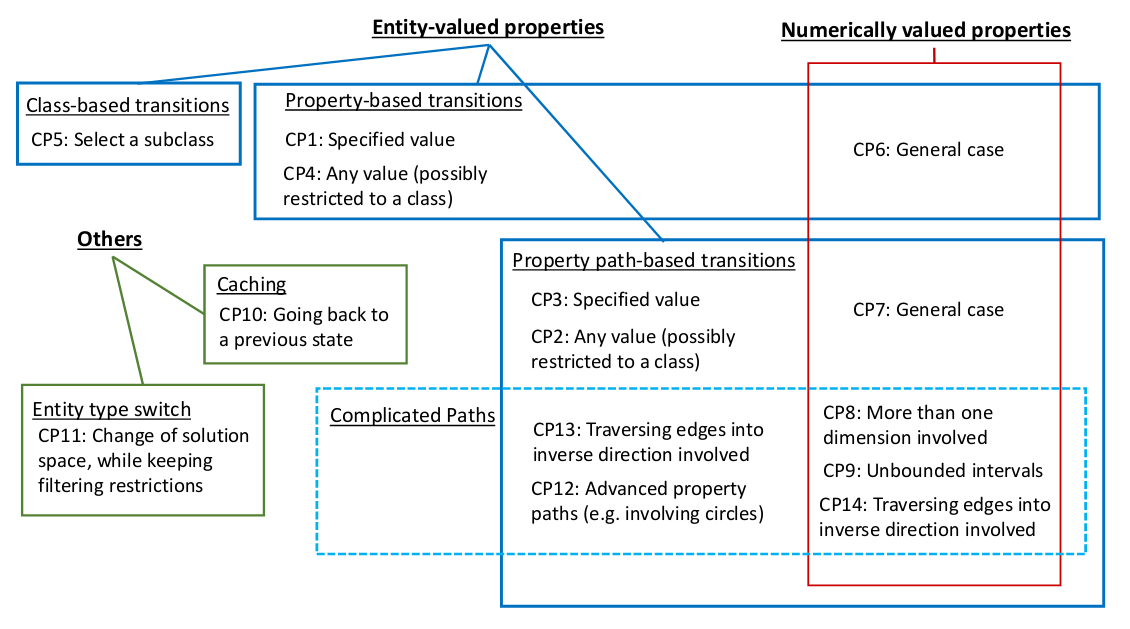
\includegraphics[width=\textwidth]{images/cps}
\caption{Overview of chokepoints}
\label{fig:chokepoints}
\end{figure}

%\todo{This list is extensible}
A chokepoint is essentially a named faceted browsing interaction followed by a subsequent information need (such as facet counts or available values), whose performance and correctness
is subject to evaluation. The obtained results define
the values of the key performance indicators of the benchmark.
An overview of the chokepoints supported by our system is depicted in~\autoref{fig:chokepoints}.
These chokepoints were proposed in~\cite{petzka}, in which they are implemented on some specific instances using parametrisation of hand-crafted SPARQL query templates. In our system, they are implemented in a generalised and universal fashion.


\begin{description}
\item[CP1] Property value based transition\\
Find all instances which, additional to satisfying all restrictions defined by the state within the browsing scenario, have a certain property value
\item[CP2] Property path based transition\\
Find all instances which additionally realise this property path with any property value
\item[CP3] Property path value based transition\\ 
Find all instances which additionally have a certain value at the end of a property path.
N.b. This is CP1 with a property path instead of a property
\item[CP4] Property class value based transition\\
Find all instances which additionally have a property value lying in a certain class
\item[CP5] Transition of a selected property value class to one of its subclasses \\
For a selected class that a property value should belong to, select a subclass
\item[CP6] Change of bounds of directly related numerical data\\
Find all instances that additionally have numerical data lying within a certain interval behind a directly related property
\item[CP7] Change of numerical data related via a property path of length strictly greater than one edge\\
Similar to 7, but now the numerical data is indirectly related to the instances via a property path
\item[CP8] Restrictions of numerical data where multiple dimensions are involved\\
Chokepoints 7 and 8 under the assumption that bounds have been chosen for more than one dimension of numerical data, here, we count latitude and longitude numerical values together as one dimension
\item[CP9] Unbounded intervals involved in numerical data\\
Chokepoints 7,8,9 when intervals are unbounded and only an upper or lower bound is chosen
\item[CP10] Undoing former restrictions to previous state\\
Go back to instances of a previous step
\item[CP11] Entity-type switch changing the solution space\\
Change of the solution space while keeping the current filter selections
\item[CP12] Complicated property paths or circles\\
Chokepoints 3 and 4 with advanced property paths involved
\item[CP13] Inverse direction of an edge involved in property path based transition\\
Property path value and property value based transitions where the property path involves traversing edges in the inverse direction
\item[CP14] Numerical inequality restriction over a property path involving the inverse direction of an edge\\
Additional numerical data restrictions at the end of a property path where the property path involves traversing edges in the inverse direction
\end{description}


\subsection{Configuration and Output}
The benchmark is configured with an RDF document describing the number of faceted search scenarios to generate as well as how many interaction/chokepoints to apply within a scenario. The application of chockepoints is controlled using a non-deterministic-automaton (NFA). This makes it possible to configure the benchmark generator to simulate natural behavior more closely. For example, this snippet in ~\autoref{fig:config-and-output} shows, that the first interaction is always the selection of a certain type. The min/max ranges are substituted with new concrete values on every scenario. The output is simply a set of RDF resources with the SPARQL query string and metadata attached.


\begin{figure}
\centering
\bgroup
\def\arraystretch{1.5}
\begin{tabular}{m{8cm}m{8cm}}
\begin{lstlisting}[language=sparql, linewidth=7cm]
:defaultScenarioConfig
  a o:ScenarioConfig ;
  o:randomSeed 1000 ;
  o:scenarioLength [ o:min 4; o:max 8;
    o:type xsd:integer] ;
  o:numScenarios 10 ;
  o:numWarmups 2 ;
  o:nfa [
    o:startState o:state1 ;
    o:transition [
      o:from o:state1 ;
      o:to o:state2 ;
      o:key "cp5" ;
      o:weight [ o:min 0.6 ; o:max 1.0 ]
    ] ;
    # More states
  ] .
\end{lstlisting}

&

\begin{lstlisting}[language=sparql, linewidth=7cm]
:scenario1-0
  o:chokepointId 5 ;
  o:queryId 0 ;
  o:scenarioId 1 ;
  o:sequenceId 0 ;
  o:task "SELECT * { ... }"
  o:expectedResult "..." ;
  o:expectedResultSize 1001 .
\end{lstlisting}

\\

\end{tabular}
\egroup
\caption{Benchmark generator configuration and output models}
\label{fig:config-and-output}
\end{figure}


\section{Evaluation}
\label{sec:evaluation}
For evaluation, we created an integration of our benchmark generator with the HOBBIT Platform\footnote{\url{http://project-hobbit.eu/}}.
HOBBIT is a benchmarking platform that follows the FAIR principles (Findability, Accessibility, Interoperability, and Reusability)\footnote{\url{https://www.nature.com/articles/sdata201618.}}.
It hosts 5 triple stores which participated in the faceted browsing challenge, namely
Apache Jena Fuseki 3.6.0, VOS for all, GraphDB Free 8.5, Virtuoso v8.0 and Blazegraph.

For benchmark data, we generated datasets using the \emph{Public Transport RDF Dataset Generator} PoDiGG~\cite{podigg}. The generated data has a small schema with main entities being stops, routes (sequences of stops) and connections (instances of routes at certain times). Using our framework, we generated a faceted browsing benchmark using a Virtuoso 7.2.5\footnote{\url{https://virtuoso.openlinksw.com/}} as the reference triple store (via the tenforce/virtuoso docker image\footnote{\url{https://github.com/tenforce/docker-virtuoso}}). The Virtuoso instance used as the reference triple store differed from the one that acted as the system under test (SUT).

The systems under tests' query execution time was limited to 5 minutes. Although we experimented with data set sizes up to 10M triples, it turned out, that even on a small data set with 500K triples, two systems were still not able to complete all queries in less than 5 minutes. \autoref{fig:eval-performance} shows the results for a setup with 234 unique queries across 322 tasks (CP10 is the undo operation, hence some duplicate queries are intentional), 24 queries were used as warm-up (which amounts to approx 20\%). All systems yielded the same result sets on all tasks, and thus performed correctly. \autoref{fig:eval-performance-cp} shows the results per chokepoint, which indicates that all of them were applied in the generated benchmark.
We also conducted experiments with DBpedia data, however, its schema graph has too many possible combination of paths. As such, we defer to future work before we can select a sensible subset of DBpedia to evaluate the path finding components on.
An interesting aspect with a DBpedia dataset with 170 million triples was, that a simple aggregation for facet values of~\autoref{lst:simple-facet} took with approximately 3min30sec the same time using a Virtuoso VOS 7.2.4 (single core) deployed on a developers' DELL XPS13 9360 notebook and a Supermicro server with 8GB and 64GB allocated to it. Hence, the aggregation is -- for this triple store -- a CPU bound operation.

\begin{figure}
\centering
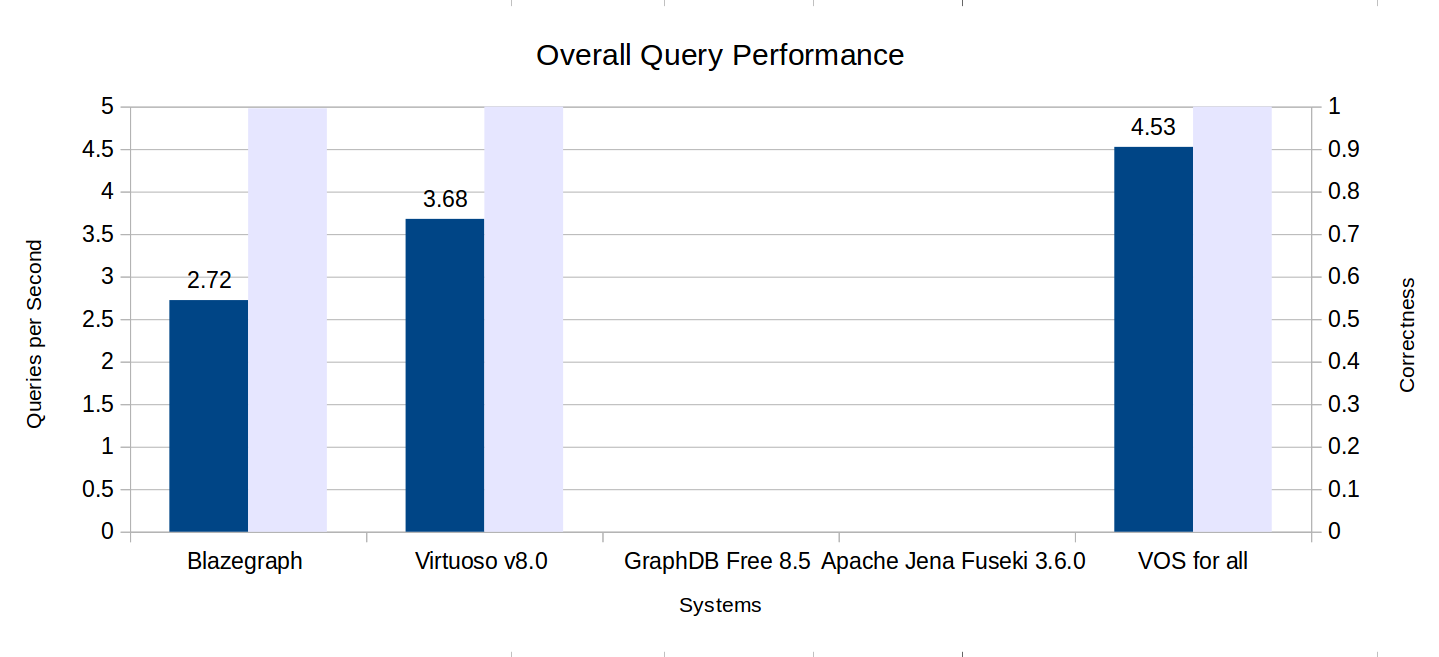
\includegraphics[width=\textwidth]{images/eval-performance-chart.png}
\caption{HOBBIT Benchmark Results on PoDiGG}
\label{fig:eval-performance}
\end{figure}

\begin{figure}
\centering
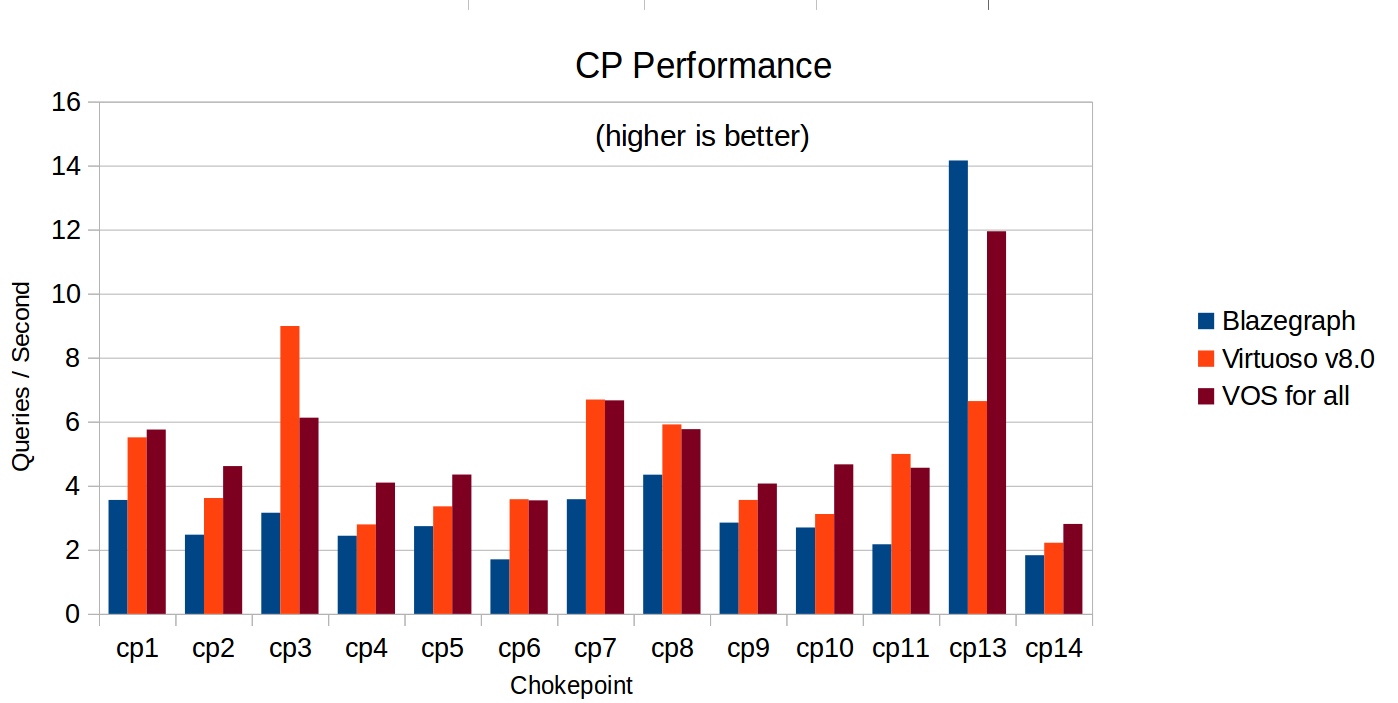
\includegraphics[width=\textwidth]{images/eval-performance-chart-cp.png}
\caption{Performance of queries by chokepoint}
\label{fig:eval-performance-cp}
\end{figure}


\section{Related Work}
\label{sec:related-work}
The first faceted search approaches were developed in the 1990s for information retrieval systems. They combined the paradigms of \textit{structured retrieval} and \textit{similarity-based ranking} by leveraging the benefits of constraint-based querying over large data sources. Since then, the approach has proven to be tremendously useful for search applications. Hence, faceted browsing is ubiquitous on the Web today. Most if not all major online applications provide at least some degree of faceted browsing feature to navigate the metadata records of their items \cite{tunkelang}.\\ 
This is why this approach has not only been applied for unstructured text documents, but also for knowledge graph data. To this date, a couple of prototypes facilitate indexing and faceted browsing of RDF data \cite{cheng, davies, hahn, waitelonis, moreno-vega}. But since these systems require an index at runtime, they offer limited flexibility regarding the kinds of queries that can be posed. Hence, entity types or facet combinations are hard-wired into the system and can not be easily adapted to changing user needs or different kinds of schemas and data models \cite{wenige}. Other approaches overcome these problems by facilitating ad-hoc exploration and facettation of RDF data from triple stores \cite{stadler, kremen, ferre, arenas}. The query-based faceted search paradigm goes back to Ferr\'{e} et al. who introduced a high level query language to integrate SPARQL querying and property-based navigation \cite{ferre}. The \textit{facete} and the \textit{SemFacet} engines \cite{arenas} have a similar approach. They offer faceted browsing capabilities for triple stores or databases that expose a SPARQL endpoint \cite{stadler}.\\
Besides enabling end user navigation, ad-hoc RDF-based faceted search also facilitates statistical inspection. In this line of research faceted exploration is also related to Online Analytical Processing (OLAP) systems since both approaches process multi-dimensional data \cite{ben-yitzhak}. But while OLAP cubes follow a predefined metadata schema, query-based facet engines are more flexible in regard to the dimensions that can be explored.\\
However, SPARQL-based ad-hoc processing comes at the cost of performance as both path traversal and aggregation operations have to be executed at runtime. Thus, there is a need for testing triple stores with regard to their fitness for out-of-the-box browsing on various data sources and schemas. 
Only then can application providers be supported in identifying suitable infrastructures (e.g. triple stores or hardware resources) as well as potential performance bottlenecks. There exists a wide variety of RDF-based facet engines. However, evaluation methods and datasets for these systems are not yet standardized \cite{tzitzikas}. Hence, there is a need for domain-independent tools to generate faceted browsing benchmarks for different use cases in order to reproduce performance tests throughout different evaluation runs \cite{moreno-vega}. Currently, a considerable amount of benchmarks is available to evaluate the general performance of triple stores (e.g., LUBM \cite{guo}, SP2 \cite{schmidt}, BSBM \cite{bizer}, WatDiv \cite{aluc} and Geographica \cite{garbis}). On the other hand, only a few attempts have been reported in the literature that evaluate RDF-based faceted browsing. For instance, Arenas et al. describe a generic approach with which their \textit{SemFacet} engine can be tested \cite{arenas}. Petzka et al. present a benchmark dataset for different faceted queries \cite{petzka}. What is currently missing, however, is a faceted browsing benchmark generator that can be configured for various schemas, data sources and hence application domains. But in order to set up a generator tool, we need an understanding of the upper bounds of ad-hoc faceted querying. Hence, it has to be investigated which query types are actually feasible for a SPARQL-based facet navigator and can still be answered within reasonable response time limits. Thus, a  meta-benchmarking is also required. To the best of our knowledge, we are the first to present a toolset on schema-agnostic (meta-)benchmarking for faceted browsing over SPARQL endpoints. 

%\section{Discussion}
%Maybe it makes sense to add such a section.
%Limitations of the benchmark - only disjunctive queries tested
%Limitations of the platform (no sparql proxy - always need to deploy -> heavy weight process, no support for caching of generated artifacts, determinism)

%\subsection{Faceted Browsing Benchmark}
%DBpedia, LGD, und Freebase


\section{Conclusions and Future Work}
\label{sec:conclusions}
In this work we presented a schema-agnostic faceted search benchmark generation framework for triple stores.
Performance of SPARQL-based faceted search depends mainly on the triple stores' capabilities of aggregating and counting data. Some benchmarked systems reached timeouts on query loads on relatively small dataset sizes. This suggests, that even today, live faceted search on SPARQL endpoints is associated with a high performance cost. As our evaluation of a simple aggregation on a large volume of data shows, interactive performance on such data is only achievable by means of indexing.
Indexing can be performed on different levels: While it is possible to cache entirely on the SPARQL level, it may be advantageous to index on the level of a language for SPARQL-based faceted search. The reason is, that simple domain specific operations, such as "yield all facet values", may result in relatively complex SPARQL queries (as shown in~\autoref{fig:engine-real-example}).
Our resource thus provides fundamental functionality for these kinds of future research:
On the one hand, creation of such an index (via SPARQL) requires assembling exactly the queries our faceted search engine generates. On the other hand, our DSL provides a high level abstraction for faceted search queries which may be suitable for use in conjunction with advanced indexing strategies.
In any case, our benchmark generator can be used to automatically evaluate faceted search over arbitrary RDF datasets in order to detect potential performance issues.

%\section*{Acknowledgements}
%This work was supported by grants from the EU H2020 Programme for the projects HOBBIT (GA no. 688227) and QROWD (GA no. 732194).

\begin{thebibliography}{99}
\bibitem{podigg} Taelman, R.; Verborgh, R.; Nies, T. D. \& Mannens, E. (2017), PoDiGG: A Public Transport RDF Dataset Generator., in Rick Barrett; Rick Cummings; Eugene Agichtein \& Evgeniy Gabrilovich, ed., 'WWW (Companion Volume)', ACM, pp. 843-844.
\bibitem{aluc} Alu\c{c} G, Hartig O, \"{O}zsu MT, Daudjee K (2014). Diversified stress testing of RDF data management systems. In: International Semantic Web Conference, pp. 197-212. 
\bibitem{arenas} Arenas M, Grau BC, Kharlamov E, Marciuška Š,  Zheleznyakov D (2016). Faceted search over RDF-based knowledge graphs. Journal of Web Semantics, 37, pp. 55-74.
\bibitem{ben-yitzhak} Ben-Yitzhak O, Golbandi N, Har'El N, Lempel R, Neumann A, Ofek-Koifman S, Yogev S. (2008). Beyond basic faceted search. In: Proceedings of the 2008 International Conference on Web Search and Data Mining, pp. 33-44. 
\bibitem{bizer} Bizer C, Schultz A (2009). The Berlin SPARQL benchmark. International Journal on Semantic Web and Information Systems (IJSWIS), 5(2), pp. 1-24.
\bibitem{cheng} Cheng G, Ge W, Qu Y (2008). Falcons: searching and browsing entities on the semantic web. In Proceedings of the 17th international conference on World Wide Web, pp. 1101-1102.
\bibitem{davies} Davies J, Weeks R (2004). QuizRDF: Search technology for the semantic web. In: Proceedings of the 37th Annual Hawaii International Conference on System Sciences.
\bibitem{ferre} Ferr\'{e} S, Hermann A (2012). Reconciling faceted search and query languages for the Semantic Web. Int. J. Metadata, Semantics and Ontologies, 7(1), pp. 37-54.
\bibitem{garbis} Garbis G, Kyzirakos K, Koubarakis M (2013). Geographica: A benchmark for geospatial RDF stores. In: International Semantic Web Conference, pp. 343-359. 
\bibitem{guo} Guo Y, Pan Z, Heflin J (2005). LUBM: A benchmark for OWL knowledge base systems. Web Semantics: Science, Services and Agents on the World Wide Web, 3(2-3), pp. 158-182.
\bibitem{hahn} Hahn R, Bizer C, Sahnwaldt C, Herta C, Robinson S, Buergle M, Scheel U (2010). Faceted wikipedia search. In: International Conference on Business Information Systems, pp. 1-11. Springer, Berlin, Heidelberg.
\bibitem{kremen} Kremen P, Saeeda L, Blaško M. (2018). Dataset dashboard–a SPARQL endpoint explorer. In: CEUR Workshop Proceedings of Fourth International Workshop on Visualization and Interaction for Ontologies and Linked Data, VOILA.
\bibitem{moreno-vega} Moreno-Vega J, Hogan A (2018). GraFa: Scalable Faceted Browsing for RDF Graphs. In: International Semantic Web Conference, pp. 301-317. Springer, Cham.
\bibitem{petzka} Petzka H, Stadler C, Katsimpras G, Haarmann B, Lehmann J (2017). Benchmarking faceted browsing capabilities of triplestores. In: Proceedings of the 13th International Conference on Semantic Systems, pp. 128-135.
\bibitem{schmidt} Schmidt M, Hornung T, Lausen G, Pinkel C (2009). SP2Bench: a SPARQL performance benchmark. In: 2009 IEEE 25th International Conference on Data Engineering pp. 222-233. 
\bibitem{stadler} Stadler C, Martin M, Auer S (2014). Exploring the web of spatial data with facete. In: Proceedings of the 23rd International Conference on World Wide Web, pp. 175-178.
\bibitem{tunkelang} Tunkelang D (2009). Faceted search. Synthesis lectures on information concepts, retrieval, and services, 1(1), pp. 1-80.
\bibitem{tzitzikas} Tzitzikas Y, Manolis N, Papadakos P (2017). Faceted exploration of RDF/S datasets: a survey. Journal of Intelligent Information Systems, 48(2), pp. 329-364.
\bibitem{waitelonis} Waitelonis J, Sack H (2012). Towards exploratory video search using linked data. In: Multimedia Tools and Applications, 59(2), pp. 645-672.
\bibitem{wenige} Wenige L, Ruhland J. Similarity-based Knowledge Graph Queries for Recommendation Retrieval. 
\end{thebibliography}


